\begin{frame}{概要}
%\initclock
%\date{\the\year 年 \the\month 月 \the\day 日 {\Large\crono}}
  \tableofcontents
\end{frame}
\section{问题背景}%one frame only
%application case
\begin{frame}
协作定位技术有着广泛的应用前景:
  \begin{columns}[T] % contents are top vertically aligned
     \column{.5\textwidth}
     \begin{figure}
     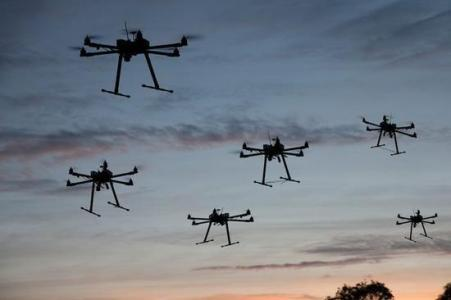
\includegraphics[height=4cm]{UAV.jpg}
     \caption*{无人机编队}
     \end{figure}
     \column{.5\textwidth}
     \begin{figure}
     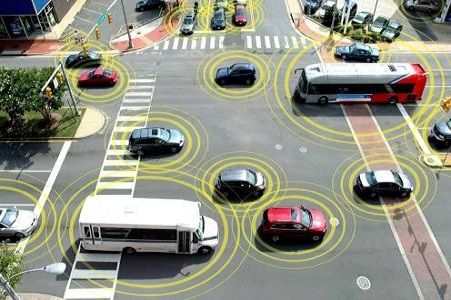
\includegraphics[height=4cm]{VL.jpg}
     \caption*{车联网}
     \end{figure}
     \end{columns}
\end{frame}
\section{数学模型}
%\subsection[非协作定位场景]{非协作定位场景}

%\subsection[协作定位场景]{协作定位场景}

%\begin{frame}{多个待测节点协作定位}
%考虑一个平面定位场景中不仅部署了$N_b$个位置已知的锚点,还有$N_a$个位置未知的待定位节点,某些位置未知的节点之间可以\alert{彼此测距},第i和第j个未知节点距离测量量服从均值为$||\bm{p}^a_i-\bm{p}^a_j||)$,方差为$\sigma_{ij}$的正态分布$X_{ij}$。
%
%以$N_a$个未知节点的位置$\{p_i^a\}$作为待估计的参数,可以得到测距量的联合概率密度函数为
%
%\begin{equation}
%\prod_{i=1}^{N_a} f(x^i_1,...x^{i}_{N_b}|\bm{p^a_i})\prod_{(i,j)\in \mathcal{E}}\frac{1}{\sqrt{2\pi\sigma^2}}exp(-\frac{(x_{ij}-f(||\bm{p}^a_i-\bm{p}^a_j||))^2}{2\sigma_{ij}^2})
%\end{equation}
%上式中$\mathcal{E}$表示可以彼此测距的未知节点的二元组的集合,而$x_t^i$表示第t个锚点和第i个未知节点的距离测量量。
%\end{frame}
%\begin{frame}{协作定位图示}
%        \begin{figure}
%          \centering
%          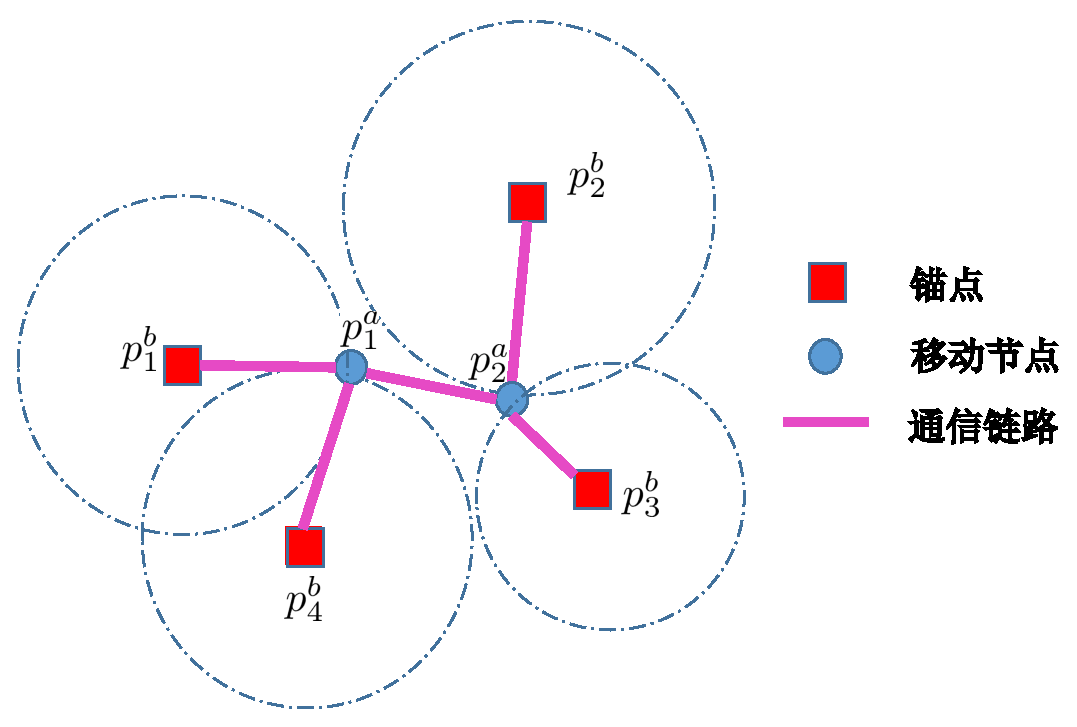
\includegraphics[width=300pt]{cooperative_spatial.eps}
%          \caption{协作静态场景下的定位}\label{fig:cooperative_spatial}
%        \end{figure}
%\end{frame}
%\begin{frame}{费舍尔信息矩阵}
%关于$2N_a$个参数$\{p_i^a\}$的费舍尔信息矩阵有如下的表达形式:
%\begin{equation}
%\scriptsize{
%I(\bm{P})=
%\left(
%\begin{array}{cccc}
%I_B(\bm{p}_1)+&-\bm{C}_{1,2}&...&-\bm{C}_{1,N_a}\\
%\sum_{j\in \{1,..N_a\}\backslash\{1\}}\bm{C}_{1,j}&&&\\
%&&&\\
%-\bm{C}_{1,2} & I_B(\bm{p}_2)+
%&...&-\bm{C}_{2,N_a}\\
%&\sum_{j\in \{1,..N_a\}\backslash \{2\}}\bm{C}_{2,j}&&\\
%&&&\\
%\vdots &\vdots&\ddots &\vdots\\
%&&&\\
%&&&I_B(\bm{p}_{N_a})+\\
%-\bm{C}_{1,N_a}&-\bm{C}_{2,N_a}&...& \sum_{j\in \{1,..N_a\}\backslash\{N_a\}}\bm{C}_{N_a,j}\\
%\end{array}
%\right)
%}
%\end{equation}
%上面的式子中$I_B(\bm{p}_i)$表示$N_b$个锚点对未知节点距离测量的贡献,和前面的(\ref{eq:uu})式相同。$C_{i,j}=\bm{1}_{(i,j)\in E}\lambda_{i,j}\bm{u}_{ij}\bm{u}_{ij}^{\textrm{T}}$,表示未知节点i和j协作的矩阵。
%$\bm{u}_{ij}=\frac{\bm{p}^a_i-\bm{p}^a_j}{||\bm{p}^a_i-\bm{p}^a_j||}$表示未知节点i和j的方向向量。
%\end{frame}
\subsection[空间协作定位]{空间协作定位}
\subsection[时间协作定位]{时间协作定位}
%\begin{frame}
%     单个节点在时间上的协作定位:
%     \begin{figure}
%          \centering
%          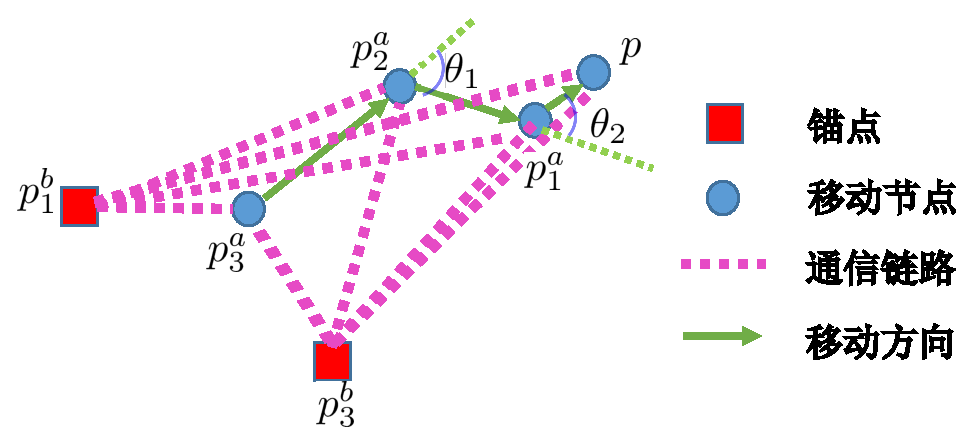
\includegraphics[height=4cm]{cooperative_single_temporal.eps}
%          \caption*{时间协作定位图示}
%     \end{figure}
%\end{frame}
\begin{frame}{数学模型}
\begin{itemize}
\item        场景中有$N_b$个位置已知的\alert{锚点}

\item        锚点在时刻$t_1,t_2,\dots,t_{N_a}$对待定位节点进行测距

\item        距离测量量服从正态分布

\item        节点在相邻时刻间可以测量速度,服从正态分布

\item        速度测量可以转化为节点相邻时刻间的距离测量
\end{itemize}
     \begin{figure}
          \centering
          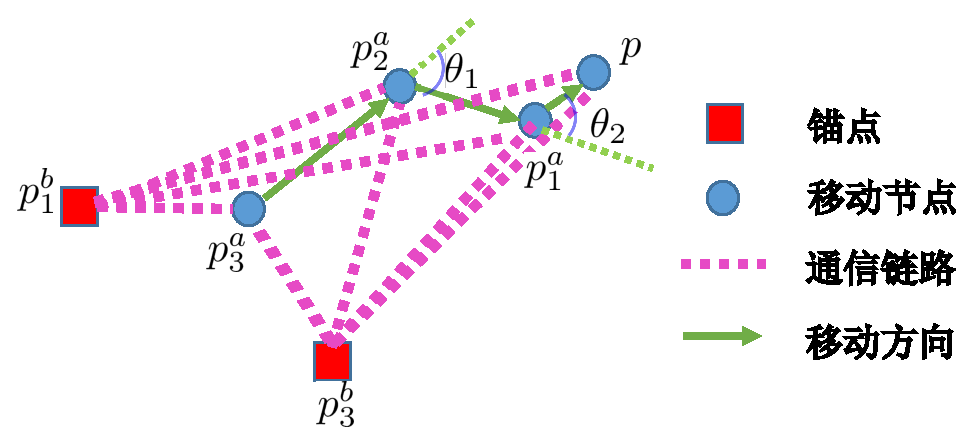
\includegraphics[height=4cm]{cooperative_single_temporal.eps}
          \caption*{时间协作定位图示}
     \end{figure}

\end{frame}
\begin{frame}
\begin{itemize}
\item 各个测量量彼此独立

\item 基于这些观测寻找对节点$\bm{p}$的位置估计最大可能的精度。

\pause
\item 根据点估计的理论,对于一个无偏估计量,它的方差的下界是\alert{费舍尔信息量}(Fisher Information)的倒数,称之为\alert{克拉美罗界}(Cram\'er-Rao Bound)。
\end{itemize}
     \begin{figure}
          \centering
          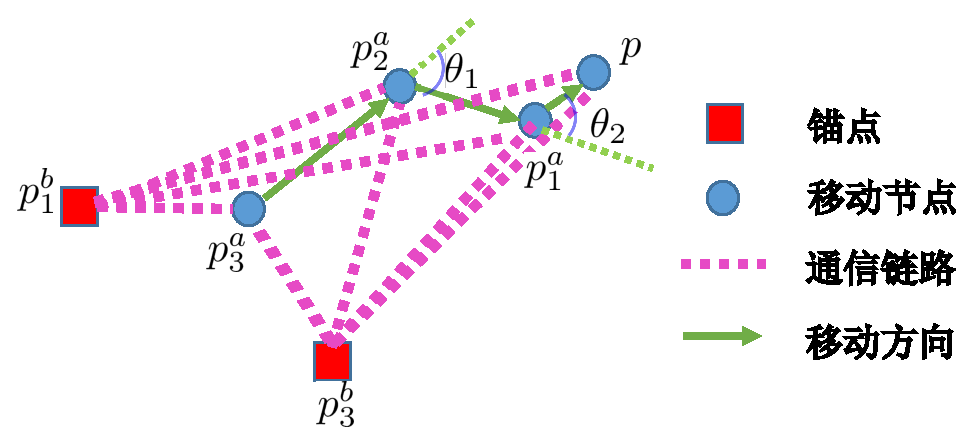
\includegraphics[height=4cm]{cooperative_single_temporal.eps}
     \end{figure}

\end{frame}
\begin{frame}
如果估计量是高维的(节点的\alert{2维}位置),费舍尔信息量推广为\alert{费舍尔信息矩阵}(Fisher Information Matrix)。


克拉美罗界在我们研究的问题中也称之为\alert{定位误差下界}(Spatial Position Error Bound),它的计算公式为:
\begin{equation*}
  \text{SPEB}=\text{tr}(\bm{I(\bm{p})}^{-1}).
\end{equation*}
     \begin{figure}
          \centering
          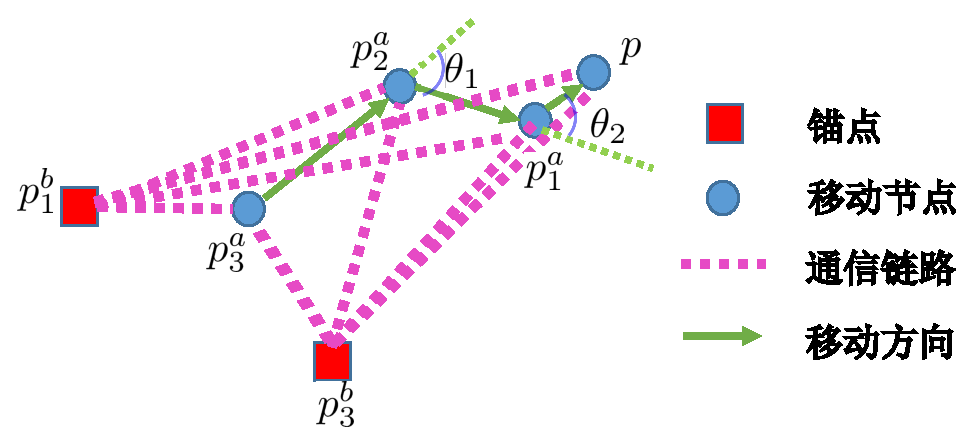
\includegraphics[height=4cm]{cooperative_single_temporal.eps}
     \end{figure}

%        \begin{figure}
%          \centering
%        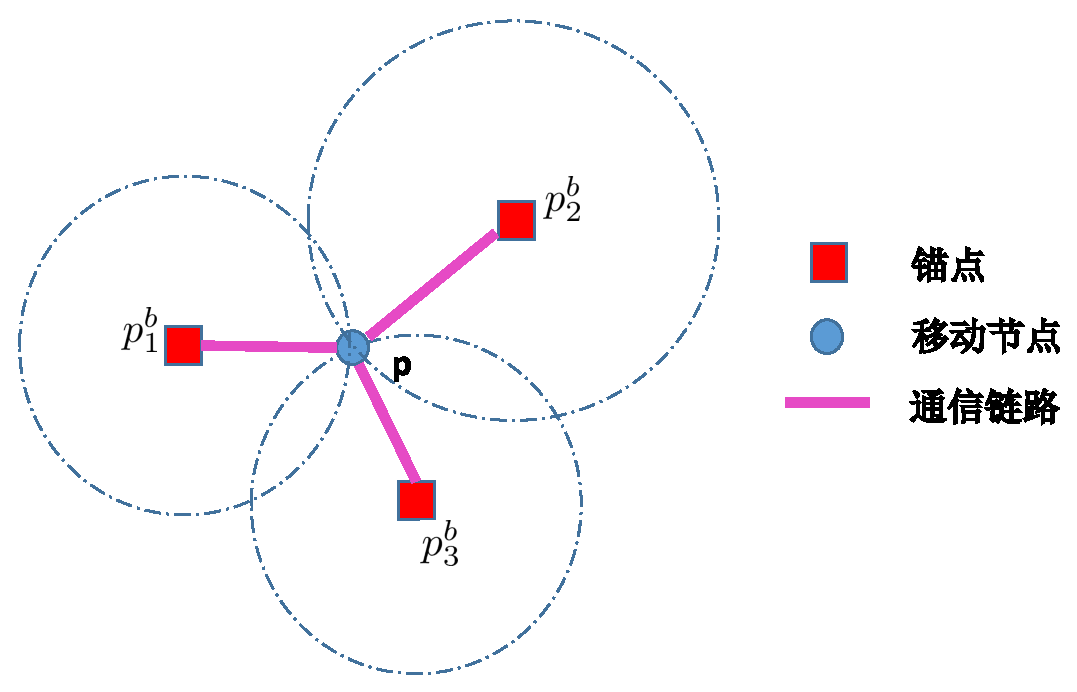
\includegraphics[width=250pt]{non_cooperative_spatial.eps}
%          \caption{非协作静态场景下的定位}\label{fig:non_cooperative_spatial}
%\end{figure}
\end{frame}

%\begin{frame}{费舍尔信息矩阵}
%以节点的\alert{2维}位置为待估计参数,费舍尔信息量推广为\alert{费舍尔信息矩阵}(Fisher Information Matrix)。
%
%对于我们的模型问题,费舍尔信息矩阵有如下的形式:
%\begin{equation}\label{eq:uu}
%I(\bm{p})=\displaystyle\sum_{i=1}^{N_b}\frac{1}{\sigma_i^2}\bm{u}_i\bm{u}_i^{\textrm{T}}
%\end{equation}
%其中
%\begin{equation}
%\bm{u_i}=\frac{\bm{p}^b_i-\bm{p}}{||\bm{p}^b_i-\bm{p}||}
%\end{equation}
%
%\end{frame}

%\begin{frame}
%假设测量时间间隔比较小使得相邻测量间节点速度方向可近似看作不变,速度测量值服从均值为$v$,方差为$\sigma_{v}$的正态分布$V_{ij}$。那么
%\end{frame}
\begin{frame}
以节点各时刻的的位置$\{p_i\}$作为待估计的参数,可以得到费舍尔信息矩阵有如下的表达形式


$\bm{I}(\bm{P})=$
\[
\begin{pmatrix}
a\bm{I}_2+&-b\bm{u}_1\bm{u}_1^{\textrm{T}}&\bm{0}&\dots&\bm{0}\\
+b\bm{u}_1\bm{u}_1^{\textrm{T}}&&&&\\
&&&&\\
-b\bm{u}_1\bm{u}_1^{\textrm{T}} & a\bm{I}_2+b\bm{u}_1\bm{u}_1^{\textrm{T}}&-b\bm{u}_2\bm{u}_2^{\textrm{T}}&\dots&\bm{0}\\
&+b\bm{u}_2\bm{u}_2^{\textrm{T}}&&&\\
\vdots &\vdots&\ddots &\vdots&\vdots\\
&&&&\\
\bm{0}&\bm{0}&...& -b\bm{u}_{N_a-1}\bm{u}_{N_a-1}^{\textrm{T}}&a\bm{I}_2+\\
&&&&+b\bm{u}_{N_a-1}\bm{u}_{N_a-1}^{\textrm{T}}\\
\end{pmatrix}.
\]
\pause
这里,费舍尔信息矩阵$\bm{I}(\bm{P})$具有块三对角的形式。
\end{frame}

%\section{简单网络}
%\subsection{非协作单节点定位网络}
%\begin{frame}{非协作单节点定位网络}
%一般的,对称正定的矩阵A定义了平面上椭圆方程$\bm{x}^{\textrm{T}}A\bm{x}=1$,
%对单节点定位误差的描述同样可以借助平面上的椭圆方程来描述:
%\begin{definition}
%对位置$\bm{p}$的2乘2的费舍尔信息矩阵$\bm{I}$定义了平面上的椭圆方程
%\begin{equation}\label{eq:ie}
%\bm{x}^{\textrm{T}}\,\bm{I}_{\bm{p}}^{-1}\bm{x}=1,\bm{x}\in \mathbb{R}^2.
%\end{equation}
%称之为节点位置的\alert{信息椭圆}。
%\end{definition}
%\pause
%信息椭圆各个主轴的长度衡量了特征值的大小,代表了该方向的定位精度。
%\end{frame}
%\begin{frame}
%对于非协作单节点定位场景,我们研究了信息椭圆离心率和定位误差下界的关系:
%\begin{figure}
%  \centering
%  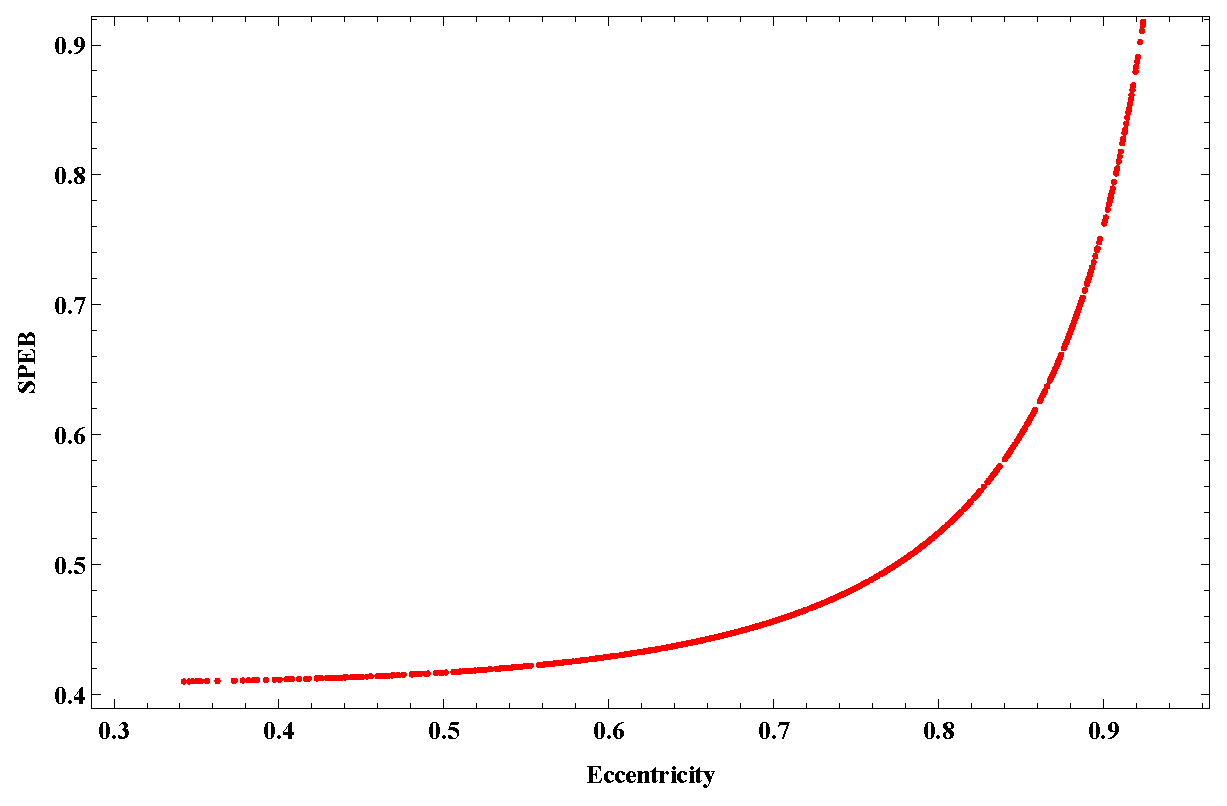
\includegraphics[width=300pt]{eccentricity_SPEB.eps}
%  \caption{定位误差下界与信息椭圆离心率的关系}\label{fig:eccentricity}
%\end{figure}
%\end{frame}
%\subsection{两个未知节点协作的场景}
%\begin{frame}
%两个移动节点协作情况下,我们可以借助下面的定理显示写出它们的位置的联合估计的费舍尔信息矩阵$I(\bm{P})$的特征多项式:
%\begin{theorem}\label{thm:ShenIden}
%设$J$是对称正定的矩阵,那么
%\begin{equation}\label{eq:ShenIden}
%|J+\epsilon \bm{u}\bm{u}^{\textrm{T}}|=|J|+\epsilon \bm{u}^{\textrm{T}}J^*\bm{u}
%\end{equation}
%其中$J^*$表示J的伴随矩阵,满足等式$JJ^*=|J|\bm{I}$
%\end{theorem}
%\pause
%借助上面的定理可以求
%\begin{equation}
%I(\bm{P})=\left(\begin{array}{cc}
%\bm{\Sigma}_0+\epsilon \bm{u}\bm{u}^{\textrm{T}}  &-\epsilon \bm{u}\bm{u}^{\textrm{T}}  \\
%-\epsilon \bm{u}\bm{u}^{\textrm{T}}  & \bm{\Sigma}_1+\epsilon \bm{u}\bm{u}^{\textrm{T}}
%\end{array}
%\right).
%\end{equation}
%的特征值。
%\end{frame}
%\section{特殊结构网络}
%\subsection{特殊的全连接网络}
%\begin{frame}{全连接网络描述与求解}
%在协作定位网络的问题模型下,给出一些简化条件后考虑$2N_a$维的联合位置估计的费舍尔信息矩阵具有如下形式:
%$I(\bm{P})=a\bm{I}_{2N}+b\bm{J}$,
%  \begin{columns}[T] % contents are top vertically aligned
%     \begin{column}[T]{5cm}
%     其中
%\[
%\bm{J}_{ij}=\begin{cases}
%\sum_{k=1,k\neq i}^N \bm{u}_{ik}\bm{u}_{ik}^{\textrm{T}}&i=j\\
%-\bm{u}_{ij}\bm{u}_{ij}^{\textrm{T}}&i\neq j
%\end{cases}
%\]
%   比如对$N=5$的情形,有$\bm{u}_{12}=\left(\cos(\frac{2\pi}{5}),\sin(\frac{2\pi}{5})\right)$
%     \end{column}
%     \begin{column}[T]{5cm}
%          \includegraphics[height=4cm]{pentagon.eps}
%     \end{column}
%     \end{columns}
%
%
%\end{frame}
%\begin{frame}
%关于矩阵$\bm{I}(\bm{P})$瑞利商为:
%\begin{equation}
%R(\bm{x})=b\sum_{i\leq j\leq N} (\bm{u}_{ij}^{\textrm{T}}(\bm{x}_i-\bm{x}_j))^2+a,\bm{x}_i\in \mathbb{R}^2
%\end{equation}
%其中$\bm{x}=(\bm{x}_1,\bm{x}_2,\dots,\bm{x}_N) \in \mathbb{R}^{2N}$且$||\bm{x}||=1$
%\pause
%
%
%容易看出,当$\bm{x}_i=\bm{x}_j$或$(\bm{x}_i-\bm{x}_j)$与$\bm{u}_{ij}$正交时,瑞利商$R(\bm{x})$取到最小值a,
%进一步可证明$I(\bm{P})$的最大特征值是$a+Nb$,且其余的特征值均为$a+Nb/2$
%\end{frame}
\section{线型网络}
\subsection{直接法}
\begin{frame}{直接法}
直接法可以给出当节点作直线运动时的平均定位误差下界:
\begin{align*}
  \text{SPEB}=&\lim_{N_a \to \infty}\frac{\tr(\bm{I(\bm{P})}^{-1})}{N_a}\\
  =&\frac{1}{a}+\frac{1}{\sqrt{a^2+4ab}}\\
\end{align*}
{\noindent 方法简述:}

$a$是$\bm{I}(\bm{P})$的$ n+1$重特征值,其余$n-1$个特征值为
\[
a+2b\left(1-\cos\frac{\pi j}{n}\right),j=1,\dots,n-1
\]
\end{frame}
%我们可以用直接法给出节点作直线运动时的平均定位误差下界:
%\pause
\begin{frame}
%$\bm{K}_{n-1}=2\bm{I}_{n-1}-\bm{S}$,由引理(\ref{lemma:special})可求出$\bm{K}_{n-1}$的全部特征值。
%\pause
\[
f(n):=\frac{\tr(\bm{I}(\bm{P})^{-1})}{n}=\frac{1}{n}\left(\frac{n+1}{a}+\sum_{j=1}^{n-1}\frac{1}{a+2b(1-\cos(\frac{\pi j}{n}))}\right)
\]
当$n\to \infty$,根据Riemann积分的定义:
\[
\lim_{n\rightarrow \infty}f(n)=\frac{1}{a}+\int_0^1 \frac{1}{a+2b(1-\cos(\pi x))}dx
\]
化为复积分由留数定理可得
\[
\lim_{n\rightarrow \infty}f(n)=\frac{1}{a}+\frac{1}{\sqrt{a^2+4ab}}.
\]
\end{frame}
\begin{frame}
$a$和${\sqrt{a^2+4ab}}$分别代表了平均定位误差下界在两个方向的信息量。


一般的,对平面上节点的位置估计的精度可以借助平面上的椭圆方程来描述:
\begin{definition}
关于位置$\bm{p}$的$2\times 2$的费舍尔信息矩阵$\bm{I}$定义了平面上的椭圆方程
\[
\bm{x}^{\textrm{T}}\,\bm{I}_{\bm{p}}^{-1}\bm{x}=1,\bm{x}\in \mathbb{R}^2.
\]
称之为节点位置$\bm{p}$的\alert{信息椭圆}。
\end{definition}
\pause
\end{frame}
\begin{frame}
信息椭圆各个主轴的长度衡量了特征值的大小,代表了该方向的定位精度。

采样时刻$N_a$很大,协作强度$b=1$,锚点定位强度$a=\lambda$:
%\the\hsize\par
%\the\vsize\par
%\the\textwidth\par
%\the\linewidth
\begin{figure}
\centering
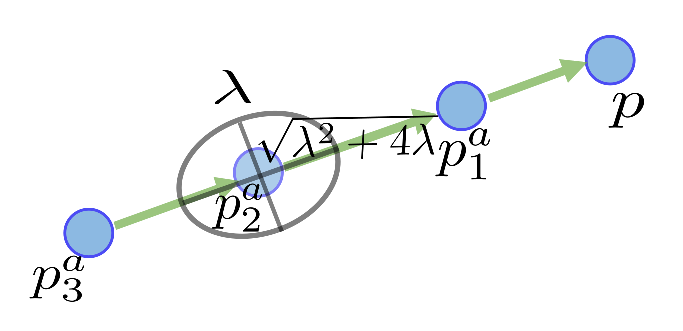
\includegraphics[width=0.8\textwidth]{direct.eps}
\caption*{信息椭圆图示}
\end{figure}
\end{frame}
%\begin{frame}{用等效费舍尔信息矩阵求解节点平均定位误差}
%给定两组数列$\{a_n\}$和$\{b_n\}$我们可以构造
%\[
%x_n=a_0+\cfrac{b_1}{a_1+\cfrac{b_2}{a_2+\dots+\cfrac{b_n}{a_n}}},\scriptsize{J=\left(
%\begin{array}{ccccccc}
%2K_1&-K_1&-K_1&0&\dots&&\\
%-K_1&2K_1&0&-K_1&0\dots&\\
%-K_1&0&2K_1&0&-K_1&0&\dots\\
%0&-K_1&0&2K_1&0&\dots&\\
%\vdots&\vdots&&\ddots&\dots&\\
%\end{array}
%\right)}
%\]
%右边的J是对节点重排后的结果,将线性网络中心的节点放到了矩阵的左上角,求解该问题还需要如下定理:
%\begin{theorem}[fundamental recurrence formulas]
%设$x_n=\frac{h_n}{k_n}$,则有如下递推关系成立:
%\vspace{-3mm}
%\begin{eqnarray}
%h_n=a_nh_{n-1}+b_nh_{n-2}\\
%k_n=a_nk_{n-1}+b_nk_{n-2}
%\end{eqnarray}
%\end{theorem}
%\end{frame}
%\begin{frame}
%为简化计算,对$a\bm{I}+b\bm{J}$提取b,记$\lambda=\frac{a}{b}$
%通过等效费舍尔信息矩阵的公式可以推导出关于矩阵$(\lambda\bm{I}+\bm{J})$左上角的2乘2矩阵的等效费舍尔信息矩阵实际是个对角阵,其中一个对角元为$\lambda$,另一个对角元为可以写成如下连分式的形式:
%\[
%\lambda+2-\cfrac{2}{\lambda+2-\cfrac{1}{\lambda+2-\cfrac{1}{\lambda+2-\dots}}}
%\]
%使用上页的定理,解常系数差分方程得通解为$\frac{h_n}{k_n}=\frac{A_1x_1^n+B_1x_2^n}{A_2x_1^n+B_2x_2^n}$
%递推公式的初始条件是
%\vspace{-2mm}
%\[
%h_0=\lambda+2,k_0=1,h_1=\lambda+2-\frac{2}{\lambda+2},k_1=\lambda+2
%\]
%其中$x_{1,2}=\frac{\lambda+2\pm \sqrt{\lambda^2+4\lambda}}{2}$
%由于$|\frac{x_1}{x_2}|>1$,所以极限$\lim_{n\to \infty}\frac{h_n}{k_n}=\frac{A_1}{A_2}$
%$A_1,A_2$可由初始条件求出,它们的比值是$\sqrt{\lambda^2+4\lambda}$
%\end{frame}
%

